\documentclass[tikz, border=15pt]{standalone}
\usepackage{tikz}
\usetikzlibrary{shapes.geometric, calc}

\definecolor{bearbody}{HTML}{D7A175}
\definecolor{bearlight}{HTML}{F6DEC4}
\definecolor{stitchcolor}{HTML}{A77043}
\definecolor{eyecolor}{HTML}{2E1C0C}
\definecolor{pawcolor}{HTML}{E8B296}
\definecolor{patchcolor}{HTML}{E66B7B}
\definecolor{patchborder}{HTML}{C54B5B}
\definecolor{blushcolor}{HTML}{F3A3A3}

\begin{document}
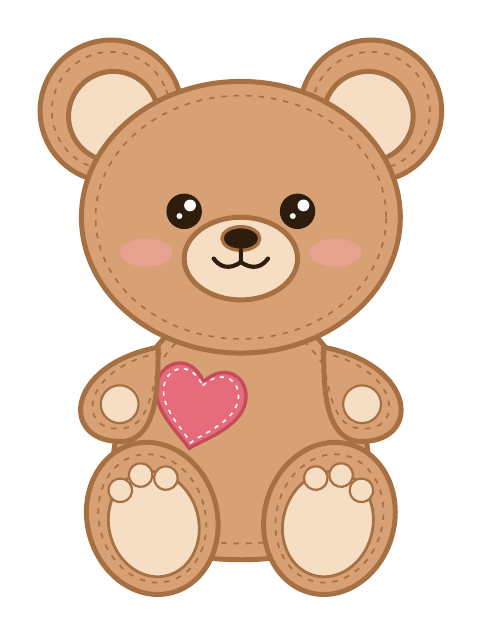
\begin{tikzpicture}[
    scale=1.5,
    every node/.style={transform shape},
    stitch/.style={draw=stitchcolor, dashed, line width=0.6pt, dash pattern=on 2pt off 2.5pt},
    outline/.style={draw=stitchcolor, line width=1.8pt, line join=round}
]

  % 1. Ears (drawn behind the head)
  % Left Ear
  \begin{scope}[shift={(-1.1, 2.1)}, rotate=25]
    \path[fill=bearbody, outline] (0,0) circle (0.6);
    \path[fill=bearlight, outline] (0,-0.05) circle (0.38);
    \path[stitch] (0,0) circle (0.5);
  \end{scope}
  
  % Right Ear
  \begin{scope}[shift={(1.1, 2.1)}, rotate=-25]
    \path[fill=bearbody, outline] (0,0) circle (0.6);
    \path[fill=bearlight, outline] (0,-0.05) circle (0.38);
    \path[stitch] (0,0) circle (0.5);
  \end{scope}

  % 2. Body (pear shape)
  \path[fill=bearbody, outline] (0, 0.5) .. controls (-0.8, 0.5) and (-1.3, -0.8) .. (-1.0, -1.4) .. controls (-0.7, -1.8) and (0.7, -1.8) .. (1.0, -1.4) .. controls (1.3, -0.8) and (0.8, 0.5) .. (0, 0.5) -- cycle;
  % Stitches for body
  \path[stitch] (0, 0.4) .. controls (-0.7, 0.4) and (-1.15, -0.75) .. (-0.88, -1.3) .. controls (-0.6, -1.65) and (0.6, -1.65) .. (0.88, -1.3) .. controls (1.15, -0.75) and (0.7, 0.4) .. (0, 0.4) -- cycle;

  % Chest patch (Stitched heart)
  \begin{scope}[shift={(-0.35, -0.35)}, scale=0.32, rotate=-12]
    \path[fill=patchcolor, draw=patchborder, line width=1.2pt] 
      (0,0.5) .. controls (0.5,1.2) and (1.2,0.8) .. (1.2,0.2)
      .. controls (1.2,-0.5) and (0.3,-1.0) .. (0,-1.3)
      .. controls (-0.3,-1.0) and (-1.2,-0.5) .. (-1.2,0.2)
      .. controls (-1.2,0.8) and (-0.5,1.2) .. (0,0.5);
    % Heart stitches
    \path[draw=white, dashed, line width=0.6pt, dash pattern=on 1.5pt off 2pt] 
      (0,0.4) .. controls (0.45,1.0) and (1.0,0.7) .. (1.0,0.2)
      .. controls (1.0,-0.4) and (0.25,-0.85) .. (0,-1.15)
      .. controls (-0.25,-0.85) and (-1.0,-0.4) .. (-1.0,0.2)
      .. controls (-1.0,0.7) and (-0.45,1.0) .. (0,0.4);
  \end{scope}

  % 3. Left Leg (sitting position)
  \begin{scope}[shift={(-0.75, -1.35)}, rotate=15]
    \path[fill=bearbody, outline] (0,0) ellipse (0.55 and 0.65);
    \path[stitch] (0,0) ellipse (0.45 and 0.55);
    \path[fill=bearlight, outline, line width=1pt] (0, -0.05) ellipse (0.38 and 0.45);
    % Toe pads
    \path[fill=bearlight, outline, line width=0.8pt] (-0.2, 0.3) circle (0.1);
    \path[fill=bearlight, outline, line width=0.8pt] (0, 0.38) circle (0.1);
    \path[fill=bearlight, outline, line width=0.8pt] (0.2, 0.3) circle (0.1);
  \end{scope}

  % 4. Right Leg
  \begin{scope}[shift={(0.75, -1.35)}, rotate=-15]
    \path[fill=bearbody, outline] (0,0) ellipse (0.55 and 0.65);
    \path[stitch] (0,0) ellipse (0.45 and 0.55);
    \path[fill=bearlight, outline, line width=1pt] (0, -0.05) ellipse (0.38 and 0.45);
    % Toe pads
    \path[fill=bearlight, outline, line width=0.8pt] (0.2, 0.3) circle (0.1);
    \path[fill=bearlight, outline, line width=0.8pt] (0, 0.38) circle (0.1);
    \path[fill=bearlight, outline, line width=0.8pt] (-0.2, 0.3) circle (0.1);
  \end{scope}

  % 5. Left Arm
  \begin{scope}[shift={(-0.7, 0.1)}, rotate=25]
    \path[fill=bearbody, outline] (0,0) .. controls (-0.8, 0.2) and (-1.1, -0.4) .. (-0.6, -0.6) .. controls (-0.3, -0.7) and (-0.1, -0.2) .. (0,0) -- cycle;
    \path[stitch] (0,-0.05) .. controls (-0.68, 0.12) and (-0.95, -0.38) .. (-0.55, -0.5) .. controls (-0.32, -0.58) and (-0.12, -0.18) .. (0,-0.05);
    \path[fill=bearlight, outline, line width=0.8pt] (-0.5, -0.3) circle (0.16);
  \end{scope}

  % 6. Right Arm
  \begin{scope}[shift={(0.7, 0.1)}, rotate=-25]
    \path[fill=bearbody, outline] (0,0) .. controls (0.8, 0.2) and (1.1, -0.4) .. (0.6, -0.6) .. controls (0.3, -0.7) and (0.1, -0.2) .. (0,0) -- cycle;
    \path[stitch] (0,-0.05) .. controls (0.68, 0.12) and (0.95, -0.38) .. (0.55, -0.5) .. controls (0.32, -0.58) and (0.12, -0.18) .. (0,-0.05);
    \path[fill=bearlight, outline, line width=0.8pt] (0.5, -0.3) circle (0.16);
  \end{scope}

  % 7. Head
  \path[fill=bearbody, outline] (0, 1.2) ellipse (1.35 and 1.15);
  \path[stitch] (0, 1.2) ellipse (1.23 and 1.03);

  % Blush (soft cheeks)
  \path[fill=blushcolor, opacity=0.55] (-0.8, 0.9) ellipse (0.22 and 0.12);
  \path[fill=blushcolor, opacity=0.55] (0.8, 0.9) ellipse (0.22 and 0.12);

  % Muzzle
  \path[fill=bearlight, outline] (0, 0.85) ellipse (0.48 and 0.35);

  % Nose
  \path[fill=eyecolor, outline, line width=1.2pt] (0, 1.02) ellipse (0.16 and 0.1);
  
  % Mouth
  \draw[draw=eyecolor, line width=1.5pt, line cap=round] 
    (0, 0.92) -- (0, 0.82)
    .. controls (-0.1, 0.75) and (-0.18, 0.78) .. (-0.23, 0.85);
  \draw[draw=eyecolor, line width=1.5pt, line cap=round] 
    (0, 0.82) 
    .. controls (0.1, 0.75) and (0.18, 0.78) .. (0.23, 0.85);

  % 8. Eyes (with cute highlights)
  % Left Eye
  \begin{scope}[shift={(-0.48, 1.25)}]
    \path[fill=eyecolor] (0,0) circle (0.15);
    \path[fill=white] (0.05, 0.05) circle (0.05);
    \path[fill=white] (-0.04, -0.04) circle (0.025);
  \end{scope}
  
  % Right Eye
  \begin{scope}[shift={(0.48, 1.25)}]
    \path[fill=eyecolor] (0,0) circle (0.15);
    \path[fill=white] (0.05, 0.05) circle (0.05);
    \path[fill=white] (-0.04, -0.04) circle (0.025);
  \end{scope}

\end{tikzpicture}
\end{document}
